\documentclass[11pt]{article}
\usepackage[margin=1in]{geometry}
\usepackage{amsmath,amssymb,amsthm}
\usepackage{graphicx}
\usepackage{booktabs}
\usepackage{xcolor}
\usepackage[numbers,sort&compress]{natbib}
\usepackage{hyperref}
\newtheorem{proposition}{Proposition}

\title{Critical Slowing Down in t-SNE Optimisation}
\author{D.~Patil}
\date{November 2026}

\begin{document}
\maketitle

\begin{abstract}
Optimising t-distributed stochastic neighbour embedding (t-SNE) takes more iterations as datasets grow. We
argue that this is \emph{critical slowing down} in the sense of statistical physics. Around an optimised
$10^5$-point embedding, the measured short-time relaxation rate of a collective displacement mode of wavenumber
$k$ grows as $k^2$, so the large-scale arrangement of the map converges far more slowly than local detail, and
shear (density-preserving) modes relax 3--4$\times$ more slowly than compression modes. We prove an exact virial
identity that certifies non-convergence along the dilation and show that the objective flattens along it. We
then test \emph{Fourier acceleration}, the standard cure for critical slowing down in lattice field theory, which
boosts the slow modes at the cost of two FFTs per iteration. In its pre-registered form (with a cap on the
optimiser's gains) it beats the better of a standard and a tuned optimiser in 11 of 15 runs on five million-point
datasets (median gain 2.1\%; the predicted 13 of 15 was not met); an uncapped variant, chosen after seeing these
results, wins 24 of 25 runs by 3.1\% on average. On nested subsets from $10^4$ to $3\times10^6$ points the capped
variant trails a tuned optimiser by 4--5\% up to $10^5$ points and leads it by 4.7\% at $3\times10^6$; it diverges in
long runs at $10^4$. A recent Nesterov optimiser \citep{lambert2023nesterov} is stronger at $10^6$ points: 2.6--3.7\%
lower KL than Fourier acceleration on four of five datasets and level on the fifth, although in our
reimplementation it inflates the map in long runs below $10^5$ points, with grid or exact repulsion. Preconditioning its gradient with the Fourier operator
makes it worse. On 1.3 million single cells Fourier acceleration has the lowest KL of the optimisers tested. We list
every sealed prediction and its outcome.
\end{abstract}

\section{Introduction}
t-SNE \citep{vandermaaten2008} remains the most widely used method for visualising high-dimensional data.
A line of work has made each iteration fast: Barnes--Hut trees \citep{vandermaaten2014bh}, interpolation and
particle--mesh FFTs \citep{linderman2019fitsne,delchevalerie2021pm,pezzotti2020gpgpu}, and GPU
implementations \citep{chan2019tsnecuda,cuml}. Far less attention has gone to the \emph{number} of
iterations. Practitioners report that large datasets need more of them \citep{belkina2019,kobak2019art}, and
default schedules compensate with larger learning rates.

We argue that the growth of the iteration count is a physical phenomenon with a known remedy. Near
convergence, a t-SNE embedding behaves like a two-dimensional elastic medium: the nearest-neighbour
attraction acts as springs, and the heavy-tailed repulsion acts as a pressure. Gradient descent relaxes a
displacement mode of wavenumber $k$ at a rate $\propto k^2$. The longest modes, in which whole regions of the
map drift, shear or expand, therefore take a number of iterations that grows with the size of the system.
This is critical slowing down \citep{hohenberg1977}. Lattice field theory cures it with Fourier acceleration
\citep{batrouni1985}, which rescales each Fourier mode of the update so that all modes relax at comparable
rates; \citet{alexander2000} carried it to off-lattice particles through a grid mapping. Optimisation theory
has an older cure, momentum \citep{polyak1964,nesterov1983}: tuned to the condition number $\kappa$, it needs about
$\sqrt\kappa$ iterations instead of $\kappa$, and with a fixed coefficient $\beta$ it speeds up slow modes by up to
$1/(1-\beta)$. We test both. Fourier acceleration improves the standard t-SNE optimiser at $10^6$ points, but the
Nesterov optimiser of \citet{lambert2023nesterov} improves it more on four of six million-point datasets, and our
attempt to combine them failed. We report this as the main empirical finding, together with the analysis.

\paragraph{Contributions.}
(i) We measure short-time relaxation rates of t-SNE optimisers around a converged $10^5$-point embedding. They
follow a $k^2$ law, and shear modes are slower than compression modes (Section~\ref{sec:csd}).
We also prove an exact virial identity at every stationary point and show that the objective flattens along the
dilation (Section~\ref{sec:theory}).
(ii) We introduce a Fourier preconditioner for t-SNE, prove that the preconditioned gradient is a descent direction
with the same stationary points, and measure its cost (Section~\ref{sec:method}).
(iii) We compare it with the standard and a tuned optimiser on five million-point datasets, two of them held
out during development and first scored under pre-registered predictions; with openTSNE and FIt-SNE;
and with two recent optimisers, the Nesterov scheme of \citet{lambert2023nesterov} and the force-normalised
swarming of \citet{lu2024swarming}, on the same affinities, including labelled benchmarks and 1.3 million single
cells (Section~\ref{sec:exp}). The Nesterov scheme is the strongest optimiser on four of the six million-point
datasets and Fourier acceleration on the single-cell data, which we cannot yet explain; we discuss the role of
bounded speed-up factors and show that preconditioning the Nesterov scheme's gradient fails
(Section~\ref{sec:momentum}).
(iv) We report where Fourier acceleration does not help: below about $10^5$ points, combined with step
normalisation, with stochastic optimisers such as UMAP's \citep{mcinnes2018umap}, and with schedules that switch it off
(Appendix~\ref{app:negative}).

\section{Background}
\paragraph{t-SNE optimisation.} Given symmetric input affinities $p_{ij}$ (perplexity 30), t-SNE minimises
$\mathrm{KL}(P\Vert Q)$ with $q_{ij}=(1+\Vert y_i-y_j\Vert^2)^{-1}/Z$. The gradient,
$4\sum_j (p_{ij}-q_{ij})(1+\Vert y_i-y_j\Vert^2)^{-1}(y_i-y_j)$, combines an attraction along the edges of the
neighbour graph with a repulsion from all points. The repulsion is computed on a grid
\citep{linderman2019fitsne,delchevalerie2021pm}. The standard optimiser uses momentum, per-coordinate
``gains'' (delta-bar-delta; \citealp{jacobs1988}), an early-exaggeration phase (attraction $\times12$ for 250 iterations), and a
learning rate of $n/12$ \citep{belkina2019,linderman2019fitsne}. openTSNE \citep{policar2024opentsne} uses
$n$ after early exaggeration. We call the FIt-SNE schedule \emph{std}. We call the best of the few standard settings
we tried (learning rates from $n/12$ to $n$, late momentum 0.8 or 0.9), learning rate $n$ and momentum 0.9 after
early exaggeration, \emph{tuned}; it is not uniformly better than \emph{std} (on GloVe-100 it is worse, and its map
width varies between seeds).

\paragraph{Fourier acceleration.} For a quadratic action on a lattice, Langevin or gradient dynamics relax
Fourier mode $k$ at a rate proportional to its stiffness $\omega(k)\propto k^2$. The slowest mode therefore
needs $O(L^2)$ steps on a lattice of side $L$. Fourier acceleration multiplies the update in Fourier space by
$\omega(k_{\max})/\omega(k)$, which equalises the rates \citep{batrouni1985}. It is used in gauge fixing
\citep{davies1988}, in Hybrid Monte Carlo and, through a particle--mesh mapping, in molecular dynamics
\citep{alexander2000}; multigrid Monte Carlo attacks the same slowing down by moving on coarse scales
\citep{goodman1986}.

\section{Critical slowing down in t-SNE}\label{sec:csd}
\paragraph{Elastic picture.} Linearise the gradient flow around a converged embedding $y^\ast$ and consider a
displacement field $u(x)=a\,\hat e\sin(k\cdot x)$. If $\hat e\perp k$ (shear), the local density is unchanged to
first order. The repulsion, a functional of the density, then does not resist the displacement: only the
neighbour springs do, with stiffness $\propto k^2$. If $\hat e\parallel k$ (compression), the repulsion adds
a pressure term. Both families are elastic at long wavelengths, so gradient descent relaxes them at rates
$\propto k^2$, shear more slowly. The springs are not Hookean: most of the $P$-weighted pairs lie beyond $s_{ij}=1$
($\langle s/(1+s)\rangle_P\approx0.8$; Section~\ref{sec:theory}), where the attractive force saturates, so the picture is
qualitative. \citet{murray2024limits} show that the attractive term of t-SNE becomes a vanishing Laplacian-type
regulariser as $n\to\infty$. In our picture this weakens the springs and slows the shear modes further as $n$
grows.

\paragraph{Measured spectrum.} We optimise a $10^5$-point embedding (Yandex Text-to-Image features) for 6000
iterations with Fourier acceleration, without a cap on the gains. This reference map is not fully converged: its KL
with the grid normaliser is 2.785, against an exact 2.709 for the tuned optimiser after 6000 iterations on the
same subset, so the rates below are measured around a map that is still relaxing. We perturb it by a single mode with $m$ wavelengths across the map ($m=1,\dots,32$). Each
optimiser then runs for 60 iterations from the perturbed embedding, with fresh gains and momentum. We
subtract an unperturbed control run and fit the decay rate of the mode's amplitude over iterations 10--60.
This measurement uses positions only, not the objective. Because gains and momentum restart with the
perturbation, these are short-time rates, not asymptotic relaxation rates: within the window the instantaneous
rate of the slowest mode still rises (under \emph{std}, from $6\times10^{-6}$ to $1.1\times10^{-5}$ per iteration
for $m=1$ shear), so we compare rates across modes and optimisers but do not extrapolate them to relaxation
times. We measured at one size only; the growth of iteration counts with $n$ is addressed by the scaling study
(Section~\ref{sec:exp}). Figure~\ref{fig:modes} and Table~\ref{tab:modes} show the result.
\begin{itemize}
\item \textbf{The $k^2$ law.} For every optimiser the rate grows as $m^{1.7\text{--}2.0}$ for $m\le8$ (fitted
log-log slopes for \emph{std}: 1.96 shear, 1.92 compression).
\item \textbf{Shear is slower than compression.} Under \emph{std}, shear modes relax 3.0--3.8$\times$ more
slowly than compression modes of the same wavelength ($m\le4$), consistent with the elastic picture, in which
only the neighbour attraction resists shear; we have not tested that mechanism separately.
\item \textbf{What Fourier acceleration does.} At this size and grid ($G=128$) the multiplier sits at its cap for
all modes with $|k|\le22.6$ grid units, so the boost is nearly uniform over the long modes: over \emph{std} it
multiplies the shear rates by 16.0, 14.4, 13.5, 12.9 and 10.5 at $m=1,2,4,8,16$, and still by 7.4 and 4.7 at
$m=24$ and 32. For compression modes the measured boost can exceed the cap (21$\times$ at $m=1$), because the
optimiser's gains and momentum respond to the preconditioned gradient: the cap bounds the operator, not the
optimiser. The tuned optimiser gets its speed from a $12\times$ larger learning rate that acts on all modes.
Because the boost is capped (Section~\ref{sec:method}), it shifts the $k^2$ law up rather than flattening it.
\end{itemize}
\begin{figure}[t]\centering
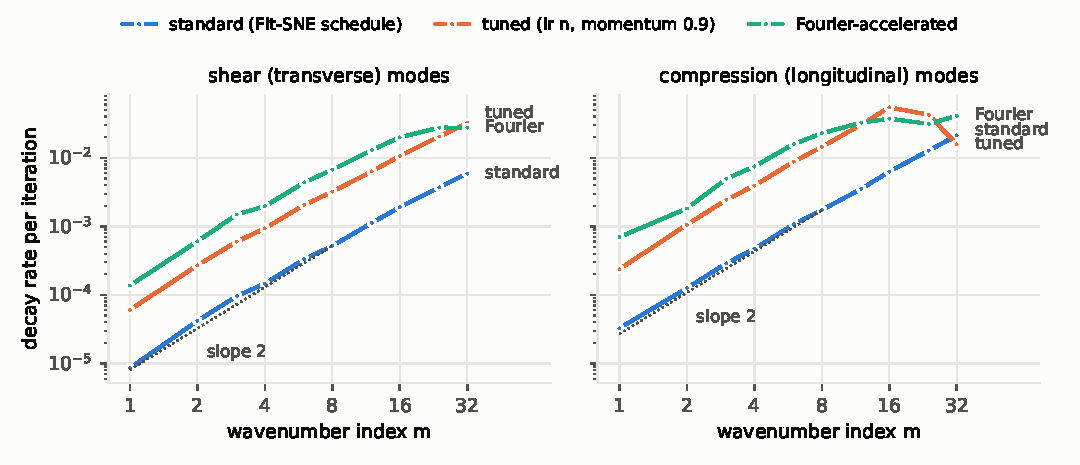
\includegraphics[width=\linewidth]{figures/modes.pdf}
\caption{Relaxation spectrum of t-SNE optimisers around a converged $10^5$-point embedding (T2I features):
decay rate per iteration of a single displacement mode with $m$ wavelengths across the map. Dotted: slope 2.}
\label{fig:modes}\end{figure}
\begin{table}[t]\centering\small
\begin{tabular}{lrrrrrr}\toprule
optimiser, polarisation & $m=1$ & $m=2$ & $m=4$ & $m=8$ & $m=16$ & $m=32$\\\midrule
standard, shear & 8.57e-6 & 4.18e-5 & 1.46e-4 & 5.19e-4 & 1.90e-3 & 5.90e-3\\
tuned, shear & 6.05e-5 & 2.70e-4 & 9.34e-4 & 3.20e-3 & 1.07e-2 & 3.24e-2\\
Fourier, shear & 1.37e-4 & 6.04e-4 & 1.97e-3 & 6.71e-3 & 1.99e-2 & 2.75e-2\\
standard, compression & 3.27e-5 & 1.26e-4 & 4.70e-4 & 1.73e-3 & 6.29e-3 & 2.12e-2\\
tuned, compression & 2.38e-4 & 1.06e-3 & 3.94e-3 & 1.45e-2 & 5.45e-2 & 1.57e-2\\
Fourier, compression & 6.99e-4 & 1.82e-3 & 7.48e-3 & 2.28e-2 & 3.72e-2 & 4.11e-2\\
\bottomrule\end{tabular}

\caption{Decay rates per iteration from Figure~\ref{fig:modes}.}\label{tab:modes}\end{table}

\section{Flat directions of the objective}\label{sec:theory}
Write $s_{ij}=\Vert y_i-y_j\Vert^2$ and $C(y)=\sum_{i\neq j}p_{ij}\log(1+s_{ij})+\log\sum_{k\neq l}(1+s_{kl})^{-1}$ (KL up
to a constant). Two exact facts about the slowest compression mode, the dilation $y\mapsto\alpha y$, and one
measurement about the long-wavelength modes help explain why these modes are slow.

\begin{proposition}[virial identity]\label{prop:virial}
At every stationary point of $C$,
$\langle s/(1+s)\rangle_P=\langle s/(1+s)\rangle_Q$, where $\langle\cdot\rangle_P$ and $\langle\cdot\rangle_Q$ average
over pairs with weights $p_{ij}$ and $q_{ij}$.
\end{proposition}
\begin{proof}
$0=\frac{d}{d\alpha}C(\alpha y)|_{\alpha=1}=\sum_i y_i\cdot\nabla_iC=2\sum_{i\neq j}(p_{ij}-q_{ij})\,s_{ij}/(1+s_{ij})$,
using $\frac{d}{d\alpha}s_{ij}(\alpha y)|_{\alpha=1}=2s_{ij}$ and $\sum_{k\neq l}(1+s_{kl})^{-2}s_{kl}\big/\sum_{k\neq l}(1+s_{kl})^{-1}=\sum q_{kl}s_{kl}/(1+s_{kl})$.
\end{proof}
\noindent With exact repulsion on 5000 SIFT points, $\langle s/(1+s)\rangle_P-\langle s/(1+s)\rangle_Q=-1.5\times10^{-2}$
after 3000 iterations and $-2.2\times10^{-3}$ after 10{,}000, and the dilation residual $\sum_iy_i\cdot\nabla_iC$ is
twice that ($-3.0\times10^{-2}$, $-4.4\times10^{-3}$), as the proof requires; meanwhile $\langle s/(1+s)\rangle_P$ grows from 0.78 to 0.86: a map
optimised for the standard 3000 iterations is still expanding. The gap is a free certificate of non-convergence along
the slowest compression mode, provided the gradient is exact: with grid repulsion the identity holds only
approximately (at $3\times10^4$ points we measured 0.754 against 0.802 for the two sides).

\begin{proposition}[the objective flattens at large scale]\label{prop:flat}
If $s_{ij}>0$ for all pairs, then as $\alpha\to\infty$,
$C(\alpha y)\to C_\infty(y)=\sum_{ij}p_{ij}\log s_{ij}+\log\sum_{k\neq l}s_{kl}^{-1}$.
\end{proposition}
\begin{proof}
$\sum p\log(1+\alpha^2s)=2\log\alpha+\sum p\log s+O(\alpha^{-2})$ and
$\log\sum(1+\alpha^2s)^{-1}=-2\log\alpha+\log\sum s^{-1}+O(\alpha^{-2})$; the $\log\alpha$ terms cancel.
\end{proof}
\noindent So along the dilation the objective tends to a constant: far out, t-SNE becomes the scale-invariant
objective $C_\infty$ with a pure $1/r^2$ kernel. A finite optimal scale therefore requires $C(\alpha y)$ to fall below
$C_\infty$ at some finite $\alpha$, which the ``$+1$'' in the Cauchy kernel makes possible; we have not characterised
when it does. This is consistent with the slow expansion above and with
the map inflation we observed at small $n$, with and without a cap on the gains and with the Nesterov scheme
(Sections~\ref{sec:exp} and~\ref{sec:momentum}). Two consequences we tested and report as negative:
solving for the scale directly from Proposition~\ref{prop:virial} is ill-posed away from equilibrium (the equation often
has no root; the iteration diverged), and minimising $C_\infty$ itself gives maps with chance-level neighbourhood
preservation (Appendix~\ref{app:negative}): the core of the kernel is what lets local structure form.

\paragraph{Tempered sampling.} We also tried to measure the flatness of the long-wavelength directions by tempered Langevin sampling. The result is inconclusive: the samplers were not at equilibrium, and two samplers of the same density disagreed 25-fold (Appendix~\ref{app:langevin}).

\section{Fourier-accelerated t-SNE}\label{sec:method}
Let $S$ spread a per-point field onto a $G\times G$ grid covering the embedding with cloud-in-cell weights, let
$D=\mathrm{diag}(S\mathbf 1)$ be the resulting point counts per node, and let $F$ be the 2-D discrete Fourier
transform. With $k_{\max}$ the largest wavenumber on the grid (its corner) and the multiplier
$M(k)=\min\!\big(c,(k_{\max}/|k|)^2\big)$ for $k\neq0$ and $M(0)=1$, the
preconditioned gradient is
\begin{equation}
  \tilde g \;=\; g + S^\top D^{-1/2}F^{-1}\,(M-1)\,F\,D^{-1/2}S\,g .
\end{equation}
\begin{proposition}\label{prop:spd}
$P=I+S^\top D^{-1/2}F^{-1}(M-1)FD^{-1/2}S$ (applied to each embedding coordinate) is symmetric and
$I\preceq P\preceq c\,I$. Hence $-\tilde g$ is a descent direction whenever $g\ne0$, and $\tilde g=0$ if and
only if $g=0$: Fourier acceleration does not change the stationary points of t-SNE.
\end{proposition}
\begin{proof}
$M$ is real, even in $k$ and satisfies $1\le M\le c$ (because $|k|\le k_{\max}$), so $B=F^{-1}(M-1)F$ is real
symmetric with eigenvalues in $[0,c-1]$. Hence $P$ is symmetric and, with $h=D^{-1/2}Sg$,
$0\le\langle g,(P-I)g\rangle=\langle h,Bh\rangle\le(c-1)\Vert h\Vert^2$. Each point's cloud-in-cell weights
are non-negative and sum to one, so $S^\top D^{-1}S$ is symmetric, non-negative and has unit row sums. It is
therefore doubly stochastic, and its spectral norm is at most 1. Hence
$\Vert h\Vert^2=\langle g,S^\top D^{-1}Sg\rangle\le\Vert g\Vert^2$, which gives $I\preceq P\preceq cI$. Then
$\langle g,\tilde g\rangle=\langle g,Pg\rangle\ge\Vert g\Vert^2>0$, and $Pg=0$ forces $g=0$.
\end{proof}
The preconditioned gradient replaces the gradient inside the unchanged optimiser (gains and momentum). There
it is multiplied by per-coordinate gains $\Gamma$, and $\Gamma P$ is not symmetric, so the descent guarantee of
Proposition~\ref{prop:spd} holds for the preconditioned gradient but not for the full update; what carries over
is that the stationary points are unchanged. It is switched on after early exaggeration; during exaggeration it
hurts (Appendix~\ref{app:negative}). We use $c=16$ and a grid of
$G=\min\!\big(512,\max(64,\,2^{\mathrm{round}(\log_2 8n^{1/4})})\big)$: 128 at $10^5$ points and 256 from
$3\times10^5$ to $3\times10^6$. In long runs at small $n$ the per-coordinate gains can grow without bound on the
boosted expansion modes and inflate the map. Capping them at 10 (with a grid of at least 128) does not prevent this:
at $10^4$ points all three capped runs were stable to 5000 iterations and then blew up (exact KL 2.6, 5.8 and 678 at
6000; Section~\ref{sec:exp}). The cap also costs 0.8--1.3\% in exact KL
at $10^6$ points on three of five datasets (Appendix~\ref{app:negative}), so the results below use no cap, and
neither variant should be run for long below about $10^5$ points. The cost is one pair of $G\times G$ FFTs and two
cloud-in-cell passes per iteration. Measured on one B200 with no other job, an iteration at $10^6$ points takes
5--7\% longer than with the \emph{tuned} optimiser (12.4--12.6 against 11.6--11.7\,s per 1000 iterations on DEEP1M,
16.1 against 15.3\,s on GloVe-100).

\section{Experiments}\label{sec:exp}
\paragraph{Protocol.} The \emph{std}, \emph{tuned} and Fourier arms share the same affinities (perplexity 30, 90 exact
neighbours), the same PCA initialisation with seeded jitter, 250 early-exaggeration iterations and grid-based
repulsion, and differ only in the post-exaggeration update. The other optimisers use the same affinities and
repulsion with their own initialisation and schedule (paragraph ``Other optimisers''). The \emph{exact} KL divergence uses the exact normaliser $Z$ over all
pairs, which we compute on the GPU in float32 tiles with float64 sums. In the runs of Table~\ref{tab:main} the grid
approximation of $Z$ used during optimisation underestimates $Z$ by 1.4--3.5\% for the wider maps that Fourier
acceleration produces, against 0.1--0.3\% for \emph{std} and 0.2--0.8\% for \emph{tuned}, except on GloVe-100, where
\emph{tuned}'s map width varies and the error ranges from a 1.3\% underestimate to a 6.1\% overestimate. KL values
computed with the grid normaliser therefore favour Fourier acceleration by up to about 3 percentage points of $Z$,
and more against two GloVe-100 \emph{tuned} runs, so every KL in our tables is exact unless labelled otherwise. We also report 10-nearest-
neighbour (10-NN) preservation on 10,000 random points, which does not depend on $Z$. Predictions were sealed
in a hash-chained ledger before each experiment ran. The two held-out datasets were first scored once, under
sealed predictions, and reused in later experiments. Hardware: one NVIDIA B200 per run; some later runs shared the
GPU with another job, and we report no timings from those.

\paragraph{Main results.} Table~\ref{tab:main} covers five datasets of about $10^6$ points: SIFT1M, DEEP1M and
GloVe-100 from ann-benchmarks, and two datasets held out during development, Yandex Text-to-Image (T2I,
images) and dbpedia OpenAI embeddings (text). Fourier acceleration ends below the better of \emph{std} and
\emph{tuned} in exact KL after 3000 iterations in 24 of 25 runs (five seeds per dataset; the exception, a GloVe-100
seed, is 0.1\% higher), by 3.1\% on average (95\% bootstrap interval 2.7--3.4\%; per run from $-6.7\%$ to $+0.1\%$), and
preserves 10 nearest neighbours better than both baselines in all 25 runs, by 1--17\% in the medians. Against
\emph{std} alone it is lower in all 25 runs. This repeats, with the exact normaliser and fresh runs, the earlier
approximate-normaliser result. Judged by exact KL at snapshots every 500 iterations, it was below the tuned
optimiser's 3000-iteration objective within 1250 post-exaggeration iterations (of 2750) in every seed on SIFT1M,
T2I and dbpedia, within 1250--2250 on DEEP1M, and within 750--1250 in four of five seeds on GloVe-100 (never in the
fifth). On GloVe-100 the tuned optimiser is worse than \emph{std} (median 6.177 against 6.145), which is why we compare
against the better baseline.

\paragraph{What was pre-registered.} The sealed predictions for this table concerned the engine with the gains cap,
not the one reported above. Against the better baseline it won in 11 of 15 runs (first three seeds), so the
prediction of at least 13 failed. The median gain was 2.1\% (predicted at least 1.5\%; held), and its 10-NN
preservation was at least the tuned optimiser's in 14 of 15 runs (held). It was not within 0.5\% of the uncapped
engine (failed). We report the uncapped engine, which was the engine of the earlier sealed held-out test, as the
headline, but we chose it after seeing this table, and we added seeds 4 and 5 afterwards: its main-table numbers
are exploratory. Table~\ref{tab:sealed} in the appendix lists every sealed prediction behind this paper and its
outcome. Not every experiment was sealed: the comparisons with other optimisers at $10^6$ points (whose first
results we saw before sealing the follow-up tests), the labelled and single-cell benchmarks, and the comparisons with
established implementations were not.
\begin{table}[t]\centering\small\resizebox{\linewidth}{!}{\begin{tabular}{lrrrlrrrr}\toprule
 & \multicolumn{5}{c}{exact KL after 3000 iterations (median of 5 seeds)} & \multicolumn{3}{c}{10-NN preservation (median)}\\
\cmidrule(lr){2-6}\cmidrule(lr){7-9}
dataset & std & tuned & Fourier & mean change vs better baseline [95\% CI] & wins & tuned & Fourier & vs best\\\midrule
SIFT1M & 5.133 & 4.967 & 4.696 & $-5.5\%$ [$-6.2$, $-4.8$] & 5/5 & 0.285 & 0.291 & $+1\%$\\
DEEP1M & 5.251 & 5.177 & 5.130 & $-1.0\%$ [$-1.5$, $-0.6$] & 5/5 & 0.199 & 0.221 & $+11\%$\\
GloVe-100 & 6.145 & 6.177 & 6.058 & $-1.8\%$ [$-3.4$, $-0.6$] & 4/5 & 0.160 & 0.169 & $+5\%$\\
T2I-1M$^\dagger$ & 4.136 & 4.023 & 3.889 & $-3.3\%$ [$-3.4$, $-3.1$] & 5/5 & 0.257 & 0.306 & $+17\%$\\
dbpedia-1M$^\dagger$ & 4.388 & 4.227 & 4.070 & $-3.8\%$ [$-4.0$, $-3.6$] & 5/5 & 0.295 & 0.348 & $+11\%$\\
\midrule
all five & & & & $-3.1\%$ [$-3.4$, $-2.7$] & 24/25 & & & \\
\bottomrule\end{tabular}
}
\caption{Main results at $\approx10^6$ points: exact KL divergence after 3000 iterations (medians over seeds); the
mean per-seed change of Fourier acceleration against the better of \emph{std} and \emph{tuned} for the same seed,
with a 95\% bootstrap interval over seeds (last row: the mean over datasets, resampling seeds within each dataset);
the number of seeds in which it is lower; and median 10-NN preservation. With five seeds the per-dataset intervals
are rough, and the pooled interval treats the five datasets as fixed. Exploratory: the sealed predictions concerned
the capped engine (see text). $\dagger$: held out during development.}\label{tab:main}\end{table}
\begin{figure}[t]\centering
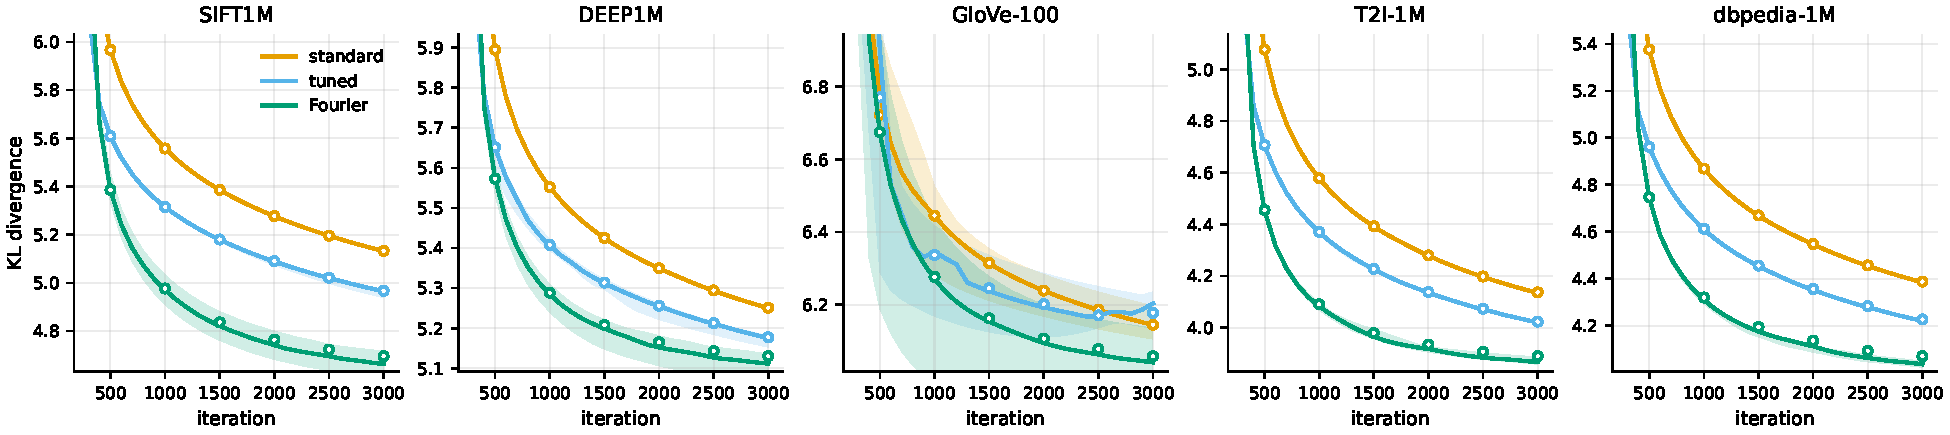
\includegraphics[width=\linewidth]{figures/kl_paper_main.pdf}
\caption{KL divergence against iteration for the runs of Table~\ref{tab:main} (five seeds). Lines: median KL with the
approximate (grid) normaliser, which biases Fourier's curve low by about 0.02--0.03; bands: range over seeds;
circles: median exact KL.}\label{fig:main}\end{figure}

\paragraph{Held-out datasets.} T2I ($10^6\times200$) and dbpedia ($10^6\times1536$) were not used during
development. In their sealed first scoring (earlier run set, approximate normaliser), Fourier acceleration was below the tuned optimiser's KL at 3000
iterations in 4 of 4 runs. It reached that objective in 950--1150 post-exaggeration iterations instead of
2750 (15--18\,s instead of 33--37\,s), and raised 10-NN preservation from 0.256 to 0.306 (T2I) and from 0.300
to 0.348 (dbpedia). All four pre-registered predictions held. With the exact normaliser and five fresh seeds the
KL gaps are $-3.3\%$ and $-3.8\%$ on average (Table~\ref{tab:main}).

\paragraph{What the embeddings look like.} Figure~\ref{fig:emb} shows the three SIFT1M embeddings after 3000
iterations (seed 0 of the earlier run set; the numbers in this paragraph come from those maps). The
Fourier-accelerated map has a diffuse rim that the others lack. On a random sample
of 20,000 points we computed the rank correlation between a point's distance from the centre of the map and
its distance to its 10th neighbour in the original 128-d space. It is $+0.26$ for Fourier against $+0.15$
for \emph{tuned} and $+0.16$ for \emph{std}. The outer 5\% of the Fourier map have a median 10th-neighbour
distance of 253, against 241 for the other two (rest of the map: 223). The rim therefore collects the
high-dimensional outliers more consistently, at the cost of a wider map.
\begin{figure}[t]\centering
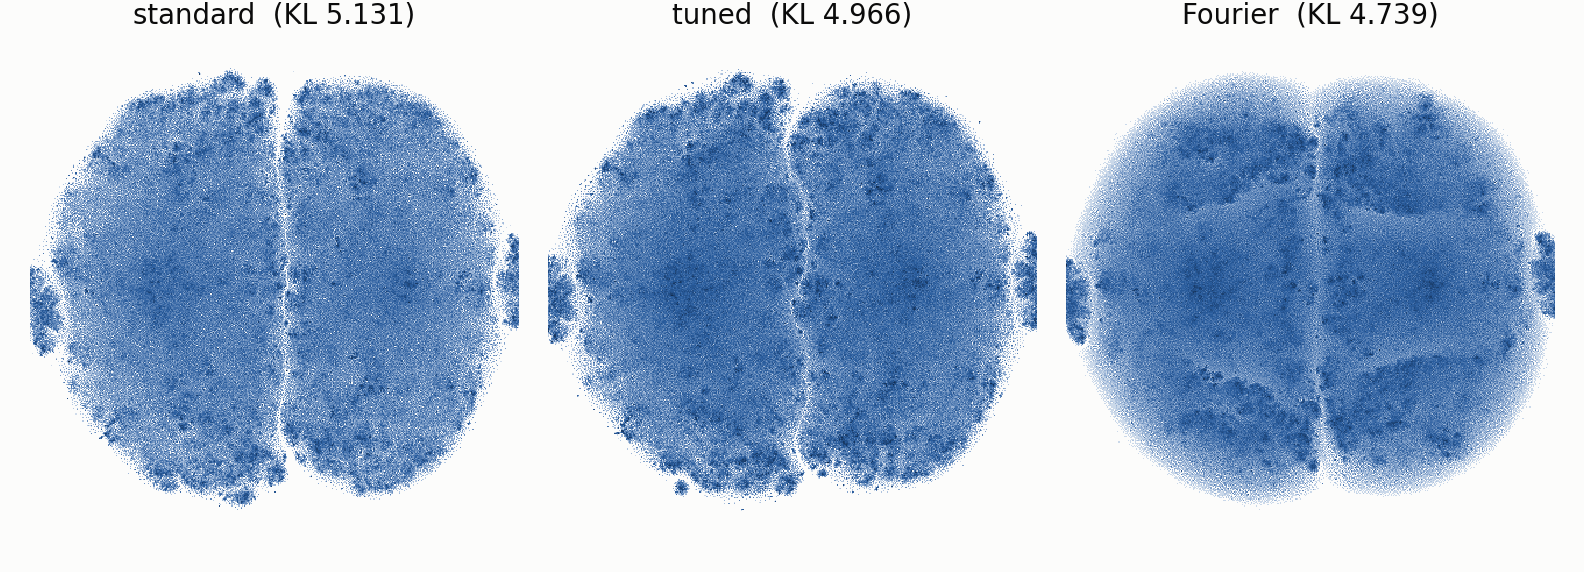
\includegraphics[width=\linewidth]{figures/emb_SIFT1M.png}
\caption{SIFT1M after 3000 iterations, seed 0 of the earlier run set (log point density). Panel titles give the KL
with the approximate normaliser; the exact values are 5.133, 4.969 and 4.776 (Table~\ref{tab:main} uses independent
runs).}\label{fig:emb}\end{figure}

\paragraph{Ablations.} Table~\ref{tab:ablate} changes one component at a time on SIFT1M and GloVe-100 (two seeds,
exact KL after 3000 iterations, the same seeds as the reference). The reference is the engine with gains capped at 10,
so the comparisons are internal to that variant. Three of seven sealed predictions held: the $1/|k|^2$ multiplier beats
a flat low-pass boost of the same cap, a cap of 64 is much worse than 16 (and unstable on GloVe-100), and momentum 0.9
is worse than 0.8. Four failed. A finer preconditioner grid ($G=512$) is 1--2\% better than 256, so our grid rule is
not optimal; $G=128$ is better on GloVe-100 and worse on SIFT1M; a cap of 4 ties 16 on GloVe-100; and shortening
early exaggeration to 100 iterations costs 2--6\%. We report these as measured and did not retune the engine after
seeing them. GloVe-100 is noisy for every variant (reference seeds 6.00 and 6.23).
\begin{table}[t]\centering\small\resizebox{\linewidth}{!}{\begin{tabular}{llrrrr}\toprule
 & & \multicolumn{2}{c}{SIFT1M} & \multicolumn{2}{c}{GloVe-100}\\
\cmidrule(lr){3-4}\cmidrule(lr){5-6}
change & sealed prediction & exact KL & vs reference & exact KL & vs reference\\\midrule
reference: $c=16$, $G=256$, $1/|k|^2$, EE 250, momentum 0.8 & & 4.688 & & 6.114 & \\
$c=4$ & worse on both (failed) & 4.876 & $+4.0\%$ & 6.103 & $-0.2\%$\\
$c=64$ & worse on one or both (held) & 5.308 & $+13.2\%$ & 7.204 & $+17.8\%$\\
$G=128$ & worse on both (failed) & 4.832 & $+3.1\%$ & 5.874 & $-3.9\%$\\
$G=512$ & within 1\% on both (failed) & 4.638 & $-1.1\%$ & 5.996 & $-1.9\%$\\
flat low-pass multiplier & worse on both (held) & 4.854 & $+3.5\%$ & 6.211 & $+1.6\%$\\
exaggeration 100 iterations & within 1\% on both (failed) & 4.773 & $+1.8\%$ & 6.448 & $+5.5\%$\\
momentum 0.9 & worse on both (held) & 4.809 & $+2.6\%$ & 6.868 & $+12.3\%$\\
\bottomrule\end{tabular}
}
\caption{Ablations at $10^6$ points: mean exact KL after 3000 iterations over two seeds, and the change against the
reference on the same seeds. The predictions were sealed before the runs.}\label{tab:ablate}\end{table}

\paragraph{Scaling.} Table~\ref{tab:scaling} runs \emph{std}, \emph{tuned} and Fourier acceleration with the gains
cap (the variant pre-registered for this study) on nested random subsets of T2I from $10^4$ to $3\times10^6$
points, three seeds each, for 6000 iterations, with exact KL. Up to $10^5$ points the capped engine trails
\emph{tuned}: after 3000 iterations by 4.3--4.5\%, with no trend. Beyond that its position improves: 1.7\% behind at
$3\times10^5$, 1.8\% ahead at $10^6$ and 4.7\% ahead at $3\times10^6$ (a sealed prediction that this ratio falls
monotonically from $10^5$ to $3\times10^6$ held). After 6000 iterations \emph{tuned} matches or beats it up to $10^6$
(+0.2\% at $10^6$), but at $3\times10^6$ it is still 3.4\% behind, and its KL after 3000 iterations (4.562) is already
below \emph{tuned}'s after 6000 (4.582). At $10^4$ every capped run diverged after 5000 iterations. So at large $n$
the capped engine gains a lead that grows with $n$; up to $10^6$ points \emph{tuned} closes it by 6000 iterations, at
$3\times10^6$ it does not. This is consistent with the growth of slow-mode costs with $n$, with two caveats: one dataset,
and a confound, since the preconditioner grid doubles from 128 to 256 between $10^5$ and $3\times10^5$ points, exactly
where the trend begins, and the ablation shows that the grid alone moves KL by 3--4\%. An earlier pass of
this study (uncapped engine, approximate normaliser) suggested $2.6\times$ fewer iterations to a target at $10^6$;
it was confounded by that normaliser's bias and by inflated runs that set the targets, and we do not use it.
\begin{table}[t]\centering\small\resizebox{\linewidth}{!}{\begin{tabular}{lrrrrrr}\toprule
$n$ & $10^4$ & $3\times10^4$ & $10^5$ & $3\times10^5$ & $10^6$ & $3\times10^6$\\\midrule
standard, 1000 it. & 2.088 & 2.501 & 3.088 & 3.744 & 4.577 & 5.406\\
tuned, 1000 it. & 2.044 & 2.414 & 2.915 & 3.543 & 4.372 & 5.203\\
Fourier, gains cap 10, 1000 it. & 2.132 & 2.490 & 2.987 & 3.509 & 4.204 & 4.883\\
\quad Fourier vs tuned & $+4.3\%$ & $+3.1\%$ & $+2.5\%$ & $-1.0\%$ & $-3.8\%$ & $-6.1\%$\\[2pt]
standard, 3000 it. & 2.031 & 2.381 & 2.843 & 3.397 & 4.134 & 4.889\\
tuned, 3000 it. & 2.014 & 2.340 & 2.758 & 3.280 & 4.022 & 4.785\\
Fourier, gains cap 10, 3000 it. & 2.103 & 2.441 & 2.882 & 3.336 & 3.950 & 4.562\\
\quad Fourier vs tuned & $+4.4\%$ & $+4.3\%$ & $+4.5\%$ & $+1.7\%$ & $-1.8\%$ & $-4.7\%$\\[2pt]
standard, 6000 it. & 2.012 & 2.320 & 2.739 & 3.247 & 3.934 & 4.648\\
tuned, 6000 it. & 2.008 & 2.320 & 2.709 & 3.174 & 3.854 & 4.582\\
Fourier, gains cap 10, 6000 it. & 5.849 & 2.449 & 2.860 & 3.289 & 3.861 & 4.428\\
\quad Fourier vs tuned & div. & $+5.6\%$ & $+5.6\%$ & $+3.6\%$ & $+0.2\%$ & $-3.4\%$\\
\bottomrule\end{tabular}
}
\caption{Scaling on nested T2I subsets (three seeds, medians): exact KL after 1000, 3000 and 6000 iterations, and
the change of Fourier acceleration (with the gains cap) against \emph{tuned}. ``div.'': diverged.}\label{tab:scaling}\end{table}

\paragraph{Established implementations.} Table~\ref{tab:external} scores openTSNE \citep{policar2024opentsne} and
the original FIt-SNE on 32 CPU cores under our affinities and metrics. Both optimise their own approximate-neighbour
affinities and are scored under ours, which puts them at a disadvantage of unknown size, and their KL values use the
grid normaliser. We also ran NVIDIA cuML \citep{cuml}, but the settings we passed had no effect (the output was
bitwise identical to its defaults), so we do not report it as a comparison. With its default 750 iterations, openTSNE's
million-point maps are far from converged (KL 5.73 on SIFT1M, 4.77 on T2I). After 3000 iterations openTSNE
reaches 5.20 on SIFT1M and 4.19 on T2I (42 minutes on 32 cores), still above both of our GPU arms. The
original FIt-SNE implementation (C++, 32 cores) ends at KL 2.86 on MNIST-70k with its default 750 iterations; at
$10^6$ points it reaches 5.85 / 5.27 (SIFT1M) and 4.88 / 4.29 (T2I) after 750 / 3000 iterations, the latter in 41
minutes end to end on 32 cores, against 4.70 and 3.89 (medians of five seeds) for the Fourier-accelerated optimiser
after about 37 seconds of optimisation on one GPU (affinities excluded).
\begin{table}[t]\centering\small\resizebox{\linewidth}{!}{\begin{tabular}{llrrr}\toprule
data & method (hardware) & KL & 10-NN & seconds end to end\\\midrule
MNIST-70k & FIt-SNE (C++), 750 it.\ (32 CPU cores) & 2.862 & 0.359 & 38\\
 & openTSNE, 750 it.\ (32 CPU cores) & 2.773 & 0.372 & 56\\
 & openTSNE, 3000 it.\ (32 CPU cores) & 2.505 & 0.389 & 1009\\
SIFT1M & FIt-SNE (C++), 750 / 3000 it.\ (32 CPU cores) & 5.847 / 5.272 & 0.178 / 0.269 & 324 / 2480\\
 & openTSNE, 750 it.\ (32 CPU cores) & 5.732 & 0.205 & 423\\
 & openTSNE, 3000 it.\ (32 CPU cores) & 5.199 & 0.280 & (2493)$^\ast$\\
 & ours: tuned / Fourier, 3000 it., median of 5 seeds (1 B200) & 4.967 / 4.696 & 0.285 / 0.291 & $\approx$36 / 38$^\ddagger$\\
T2I-1M & FIt-SNE (C++), 750 / 3000 it.\ (32 CPU cores) & 4.877 / 4.291 & 0.165 / 0.241 & 375 / 2478\\
 & openTSNE, 750 it.\ (32 CPU cores) & 4.770 & 0.176 & 440\\
 & openTSNE, 3000 it.\ (32 CPU cores) & 4.186 & 0.256 & 2520\\
 & ours: tuned / Fourier, 3000 it., median of 5 seeds (1 B200) & 4.023 / 3.889 & 0.257 / 0.306 & $\approx$34 / 37$^\ddagger$\\
\bottomrule\end{tabular}
}
\caption{Established implementations under our affinities and metrics. External embeddings are scored with the
grid normaliser, whose error in our own runs was at most 0.035 in KL (0.06 for two unstable \emph{tuned} runs), well
below the gaps in this table; our rows use exact KL and repeat Table~\ref{tab:main}. $^\ast$Timing contaminated by a concurrent CPU job; not used. $^\ddagger$Optimisation only: our affinities use an exact GPU $k$-NN search (25--90\,s at $10^6$
points) that an approximate search would shorten.}\label{tab:external}\end{table}

\paragraph{Other optimisers.} Table~\ref{tab:competitors} runs two recent optimisers on the same affinities, grid
repulsion and 3000 iterations: the Nesterov scheme of \citet{lambert2023nesterov} (momentum 0.995, gradient
rescaled to a fixed norm $\sqrt{2n}/100$, no early exaggeration, whitened PCA initialisation) and the
attraction--repulsion swarming of \citet{lu2024swarming} (row-normalised attraction, per-point normalised
repulsion, step 1). On these five datasets the Nesterov scheme is the strongest optimiser we tested. Its exact KL is
2.6--3.7\% below Fourier acceleration's on SIFT1M, DEEP1M, T2I and dbpedia and level on GloVe-100 (6.056 against
6.058), and it preserves more nearest neighbours on all five. A $4096^2$ repulsion grid changes it by 0.2\% or
less. Its initial jitter is $10^{-3}$ of the PCA scale (0.1 for our arms), so its three seeds are nearly the same run
(SIFT1M: 4.5196--4.5198). Swarming ends far higher (KL 5.4--6.8), but it does not minimise KL, so this measures
how far its maps are from the t-SNE optimum, not how well it does its own job. Adding Fourier acceleration to the
Nesterov scheme, by preconditioning the gradient before the rescaling, made it 11--22\% worse and cut its 10-NN
preservation by 33--47\% on every dataset (a sealed prediction that it would help failed;
Section~\ref{sec:momentum}).
\begin{table}[t]\centering\small\resizebox{\linewidth}{!}{\begin{tabular}{lrrrrrr}\toprule
exact KL / 10-NN & tuned & Fourier (ours) & Nesterov (Lambert et al.) & Nesterov, $4096^2$ grid & Nesterov + Fourier & ARS (Lu \& Calder)\\\midrule
SIFT1M & 4.967 / 0.285 & 4.696 / 0.291 & 4.520 / 0.303 & 4.530 / 0.306 & 5.073 / 0.160 & 6.208 / 0.189\\
DEEP1M & 5.177 / 0.199 & 5.130 / 0.221 & 4.997 / 0.228 & 5.006 / 0.229 (2) & 5.571 / 0.138 & 6.086 / 0.103\\
GloVe-100 & 6.177 / 0.160 & 6.058 / 0.169 & 6.056 / 0.174 & -- & 6.796 / 0.105 & 6.838 / 0.103\\
T2I-1M$^\dagger$ & 4.023 / 0.257 & 3.889 / 0.306 & 3.753 / 0.313 & -- & 4.407 / 0.211 & 5.403 / 0.163\\
dbpedia-1M$^\dagger$ & 4.227 / 0.295 & 4.070 / 0.348 & 3.929 / 0.358 & -- & 4.784 / 0.230 & 5.618 / 0.205\\
\bottomrule\end{tabular}
}
\caption{Optimisers at $\approx10^6$ points on the same affinities and repulsion: median exact KL after 3000
iterations / median 10-NN preservation. \emph{tuned} and Fourier as in Table~\ref{tab:main}; the others three
seeds (two where marked). The $4096^2$-grid variant was run only where it might matter and dropped once it did
not.}\label{tab:competitors}\end{table}

\paragraph{Labelled data.} On MNIST and Fashion-MNIST (70{,}000 points each, three seeds), every optimiser except the
Nesterov--Fourier combination gives the same $k$-NN classification accuracy in the map (0.968--0.971 on MNIST,
0.842--0.853 on Fashion-MNIST) and similar trustworthiness (0.974--0.987; Table~\ref{tab:labelled}). At this size the
tuned optimiser has the lowest KL on MNIST and the Nesterov scheme with a fine grid on Fashion-MNIST; Fourier
acceleration is within 0.25\% of the tuned optimiser on both and 1.8\% above the best on Fashion-MNIST, consistent
with its benefit appearing only at large $n$. The combination is far worse at this size (KL 4.3--4.7, accuracy
0.73--0.82).
\begin{table}[t]\centering\small\resizebox{0.9\linewidth}{!}{\begin{tabular}{llrrrr}\toprule
data & optimiser & exact KL & 10-NN & $k$-NN accuracy & trustworthiness\\\midrule
MNIST-70k & standard & 2.575 & 0.383 & 0.971 & 0.9805\\
 & tuned & 2.488 & 0.382 & 0.970 & 0.9790\\
 & Fourier (ours) & 2.494 & 0.377 & 0.968 & 0.9736\\
 & Fourier, gains cap 10 & 2.507 & 0.377 & 0.968 & 0.9738\\
 & Nesterov (Lambert et al.) & 2.586 & 0.381 & 0.968 & 0.9736\\
 & Nesterov, $4096^2$ grid & 2.503 & 0.384 & 0.968 & 0.9787\\
 & Nesterov + Fourier & 4.681 & 0.151 & 0.819 & 0.8781\\
 & ARS (Lu \& Calder) & 3.353 & 0.334 & 0.969 & 0.9790\\
Fashion-70k & standard & 2.395 & 0.351 & 0.852 & 0.9874\\
 & tuned & 2.309 & 0.354 & 0.852 & 0.9873\\
 & Fourier (ours) & 2.307 & 0.348 & 0.850 & 0.9853\\
 & Fourier, gains cap 10 & 2.316 & 0.349 & 0.852 & 0.9849\\
 & Nesterov (Lambert et al.) & 2.301 & 0.350 & 0.851 & 0.9860\\
 & Nesterov, $4096^2$ grid & 2.266 & 0.352 & 0.853 & 0.9867\\
 & Nesterov + Fourier & 4.310 & 0.133 & 0.730 & 0.9429\\
 & ARS (Lu \& Calder) & 3.153 & 0.302 & 0.842 & 0.9844\\
\bottomrule\end{tabular}
}
\caption{Labelled benchmarks (70{,}000 points, three seeds, medians): exact KL, 10-NN preservation, accuracy of a
10-NN classifier in the map (10{,}000 query points), and trustworthiness ($k=10$).}\label{tab:labelled}\end{table}

\paragraph{Single-cell data.} The 10x Genomics dataset of 1.3 million mouse brain cells \citep{10x2017neurons} is
the largest we tested (library-size normalisation, $\log(1+x)$, the 1000 most variable genes, 50 principal
components; labels from 10x's own graph-based clustering, 60 clusters). Here Fourier acceleration has the lowest
KL of all optimisers (4.883, against 4.951 for the Nesterov scheme and 5.093 for \emph{tuned}; two seeds each), the
same 10-NN preservation as the Nesterov scheme (0.210) and the same classification accuracy (0.815--0.818;
Table~\ref{tab:singlecell}). So the Nesterov scheme leads on four of the six million-point datasets, the two tie on
GloVe-100, and Fourier acceleration leads on the single-cell data. Adding Fourier acceleration to the Nesterov scheme
fails here too (KL 5.464). Two caveats on the label metrics: the 10x labels come from a clustering of the same
expression data, so classification accuracy in the map is partly circular; and trustworthiness is computed within a
random subset of 10{,}000 points, which at $1.3\times10^6$ points probes neighbourhoods of roughly the 1300 nearest
neighbours rather than the 10 nearest.
\begin{table}[t]\centering\small\resizebox{0.9\linewidth}{!}{\begin{tabular}{llrrrr}\toprule
data & optimiser & exact KL & 10-NN & $k$-NN accuracy & trustworthiness\\\midrule
10x-1.3M & standard & 5.156 & 0.163 & 0.814 & 0.9830\\
 & tuned & 5.093 & 0.177 & 0.816 & 0.9810\\
 & Fourier (ours) & 4.883 & 0.210 & 0.815 & 0.9757\\
 & Fourier, gains cap 10 & 4.957 & 0.209 & 0.815 & 0.9757\\
 & Nesterov (Lambert et al.) & 4.951 & 0.210 & 0.818 & 0.9771\\
 & Nesterov + Fourier & 5.464 & 0.127 & 0.772 & 0.9429\\
 & ARS (Lu \& Calder) & 6.025 & 0.070 & 0.802 & 0.9703\\
\bottomrule\end{tabular}
}
\caption{10x Genomics 1.3M mouse brain cells (PCA-50): medians of two seeds; columns as in
Table~\ref{tab:labelled}.}\label{tab:singlecell}\end{table}

\section{Momentum: a hypothesis}\label{sec:momentum}
\paragraph{Why momentum might win.} For a quadratic mode with stiffness $\lambda_k\propto k^2$, gradient descent with
step $\eta$ needs about $1/(\eta\lambda_k)$ iterations, so the slowest mode costs about the condition number
$\kappa=\lambda_{\max}/\lambda_{\min}$, which grows with the size of the map. Momentum tuned to the problem,
$\beta\approx1-\sqrt{\eta\lambda_{\min}}$, would need about $\sqrt\kappa$ iterations \citep{polyak1964,nesterov1983},
but none of the schemes we tested tunes $\beta$ to $\kappa$. With a fixed $\beta$, an overdamped slow mode
($\eta\lambda\ll(1-\beta)^2$) relaxes at about $\eta\lambda/(1-\beta)$, a speed-up of up to $1/(1-\beta)$: 5 for the
standard schedule's momentum of 0.8, 10 for \emph{tuned}'s 0.9 and 200 for the 0.995 of \citet{lambert2023nesterov}.
The Nesterov scheme's large factor for slow modes is a plausible reason for its lead at $10^6$ points. We offer this
only as a hypothesis, for three reasons. The per-coordinate gains of the other optimisers are unbounded and respond to
the gradient, so their effective step is not fixed (the measured compression boost of Fourier acceleration exceeds
its cap; Section~\ref{sec:csd}). The Nesterov scheme's step normalisation makes its effective step grow as the
gradient shrinks. And simple bookkeeping of the factors mispredicts the one ordering we measured: Fourier acceleration
(cap 16, momentum 0.8) relaxes the slowest shear mode 2.3 times faster than \emph{tuned} (learning rate $12\times$,
momentum 0.9). Measuring the Nesterov scheme's relaxation spectrum would test the hypothesis directly; we have not
done so.

\paragraph{A sealed test, and why it is weak.} We predicted, before running it, that on the nested T2I subsets of the
scaling study the Nesterov scheme's gap to the best of the other three optimisers would shrink monotonically from
$10^4$ to $10^6$ points, show no real advantage at $10^4$, and reach at least $-2\%$ at $10^6$. All three predictions
held (Table~\ref{tab:lambertscaling}): $+129\%$, $+93\%$, $-1.3\%$, $-4.3\%$ and $-5.0\%$ after 3000 iterations. The
test is weaker than this suggests. At $10^4$ and $3\times10^4$ points our reimplementation of the scheme, with grid
repulsion, inflates the map (its fixed-length steps can be amplified about 200-fold by the momentum, to up to 2.8
units per point per iteration at any $n$): at $10^4$ after about 1000 iterations, to an extent of 625 against 98--156
for \emph{std} and \emph{tuned}, with KL rising from about 2.0 to 4.5; at $3\times10^4$ after about 2000 iterations, to
823. This is not an artefact of the grid: with exact repulsion on SIFT prefixes (seed 0, 6000 iterations) the map
inflates further, to an extent of 503 after 1000 iterations and about 2470 after 2000 at $10^4$ points, and from 406
to about 3050 at $3\times10^4$ (beyond an extent of about 2000 even our float32 evaluation of the exact KL breaks down,
so we report extents). A 20{,}000-point MNIST run with exact repulsion had reached a normal KL (1.95) after 2000
iterations, before inflating. The behaviour is consistent with momentum carrying the map past its optimal scale along
the flat dilation of Proposition~\ref{prop:flat}, where little pulls it back. At $10^5$ the scheme's KL is lowest after 2000 iterations and rises afterwards (2.715 to 2.861 at 6000).
At 1000 iterations the gaps at $10^5$, $3\times10^5$ and $10^6$ are $-6.0\%$, $-7.6\%$ and $-6.2\%$, not monotone. And
the comparison arm at $10^6$ is the capped engine; the uncapped one was not run in this study. Only $3\times10^5$ and
$10^6$ are clean ($-4.3\%$, $-5.0\%$), too few to establish a trend. At 70{,}000 points the picture is mixed rather
than a clear deficit: the scheme trails \emph{tuned} by 3.9\% on MNIST (0.6\% with a $4096^2$ repulsion grid) and
leads it by 0.3\% on Fashion-MNIST (1.8\% with that grid). Because the grid spacing grows with the span of the map,
wide maps get coarser repulsion, which confounds comparisons at small $n$. A step schedule would be needed to use the
scheme below $10^5$ points.
\begin{table}[t]\centering\small\resizebox{\linewidth}{!}{\begin{tabular}{lrrrrr}\toprule
$n$ & $10^4$ & $3\times10^4$ & $10^5$ & $3\times10^5$ & $10^6$\\\midrule
best of std / tuned / Fourier, 3000 it. & 2.014 & 2.340 & 2.758 & 3.280 & 3.950\\
Nesterov \citep{lambert2023nesterov}, 3000 it. & 4.620 & 4.511 & 2.722 & 3.139 & 3.752\\
change & $+129\%$ & $+93\%$ & $-1.3\%$ & $-4.3\%$ & $-5.0\%$\\
change after 6000 it. & $+125\%$ & $+91\%$ & $+5.6\%$ & $-1.2\%$ & $-4.8\%$\\
Nesterov map extent (others) & 625 (98--156) & 823 & 784 & 636 & 654\\
\bottomrule\end{tabular}
}
\caption{Nesterov scheme against the best of \emph{std}, \emph{tuned} and Fourier acceleration (with gains cap) on nested
T2I subsets: median exact KL over three seeds and relative change. Below $10^5$ points the scheme inflates the map
(last row: mean RMS extent over seeds; in brackets, \emph{std} and \emph{tuned}).}\label{tab:lambertscaling}\end{table}

\paragraph{Why the two do not combine.} The scheme of \citet{lambert2023nesterov} rescales every step to a fixed
length. Boosting the slow components of the gradient by up to $c$ before that rescaling shrinks the fast, local
components by the same factor, so local structure converges up to $c$ times more slowly. The data agree: with the
boost, 10-NN preservation fell from 0.303 to 0.160 on SIFT1M and from 0.358 to 0.230 on dbpedia. A combination would
have to apply the boost without the normalisation; we have not tested one. We also cannot explain why Fourier
acceleration leads on the single-cell data; its maps there are wider than the Nesterov scheme's (extent 484--494
against 366), which may interact with the grid repulsion in either direction.

\section{Related work}
Per-iteration accelerations of t-SNE \citep{vandermaaten2014bh,linderman2019fitsne,pezzotti2020gpgpu,
chan2019tsnecuda} are complementary to ours. The closest in spirit is PM-t-SNE \citep{delchevalerie2021pm},
which brings the particle--mesh method of physics to t-SNE. It uses FFTs on a grid to compute the repulsive
potential, as our grid repulsion does, but it does not modify the update. Other work changes the optimiser
itself: Nesterov momentum with gradient normalisation in place of early exaggeration
\citep{lambert2023nesterov}, and force-normalised attraction--repulsion swarming with a size-independent time
step \citep{lu2024swarming}. \citet{iwasaki2025accelerated} analyse Nesterov-accelerated t-SNE in continuous
time through the graph-Laplacian modes that govern cluster formation in the early phase. Multilevel
strategies embed a sample and prolong it \citep{skrodzki2023perplexity}, or optimise UMAP within growing
graph-spectral subspaces \citep{spectral2026multiscale}. Partial-Hessian strategies precondition with the
Laplacian of the input neighbour graph \citep{vladymyrov2012}. All of these act on the input graph, whereas
we precondition on the spatial modes of the embedding plane, which costs two FFTs per iteration. The closest
prior operator is Laplacian smoothing gradient descent \citep{osher2022lsgd}, which multiplies the gradient by
$(I-\sigma\Delta)^{-1}$ through an FFT over the index of the parameter vector; ours acts on the two-dimensional
spatial modes of the map through a particle--mesh mapping, with a capped $1/k^2$ multiplier. The family of low-pass,
inverse-Laplacian preconditioners is older still:
Sobolev gradients for active contours \citep{sundaramoorthi2007}, kernel-smoothed particle updates in Stein
variational gradient descent \citep{liu2016svgd}, Laplacian reparametrisations of mesh vertices
\citep{nicolet2021largesteps}, and graph-Laplacian preconditioning of centroidal Voronoi tessellations
\citep{hateley2015cvt}. Theoretical analyses of t-SNE have studied early exaggeration and cluster recovery
\citep{linderman2019provably,arora2018analysis,cai2022foundations} and large-data limits of the objective
\citep{murray2024limits}, and the attraction--repulsion balance across neighbour-embedding methods
\citep{boehm2022attraction}; initialisation strongly affects the global layout \citep{kobak2021initialization}.
\citet{belkina2019} studied how iteration counts and learning rates should grow with $n$; to our knowledge, the
relaxation spectrum of t-SNE optimisers has not been measured before.

\section{Limitations}
\begin{itemize}
\item \textbf{The evidence for critical slowing down is indirect.} We measured short-time rates at one size
($10^5$ points); the growth of relaxation times with $n$ is inferred from the $k^2$ law and from iteration counts,
not measured mode by mode, and the Nesterov scheme's spectrum was not measured.
\item \textbf{No valid uncertainty measurement.} Our tempered-sampling study was not at equilibrium and its two
samplers disagreed, so we report it only as inconclusive (Appendix~\ref{app:langevin}).
\item \textbf{The cap limits the boost.} With $c=16$ (larger caps were unstable), the $k^2$ law is shifted
rather than removed, so critical slowing down will reappear at sizes beyond those tested.
\item \textbf{The benefit needs large $n$.} In the scaling study the tuned optimiser matches or beats the capped
engine up to $3\times10^5$ points after 3000 iterations, and up to $10^6$ points after 6000.
\item \textbf{Unstable in long runs at small $n$.} At $10^4$ points the map inflates or diverges in long runs, with
or without a cap on the gains; the cap also costs up to 1.3\% in KL at $10^6$ points.
\item \textbf{Thin evidence in places.} The single-cell lead (1.4\%) rests on two seeds and no fine-grid run of the
Nesterov scheme, whose three seeds per dataset are nearly the same run; the scaling trend uses one dataset and is
confounded by a change of grid.
\item \textbf{The headline engine was chosen after seeing the results} of the corrected main table, whose sealed
predictions concerned the capped engine (Section~\ref{sec:exp}).
\item \textbf{Not the best optimiser.} At $10^6$ points the Nesterov scheme of \citet{lambert2023nesterov} reaches
2.6--3.7\% lower KL than Fourier acceleration on four of six datasets (Fourier acceleration leads on the single-cell
data, and they tie on GloVe-100), and the two do not combine as we tried them.
Fourier acceleration's margins over the standard optimiser are modest (up to 6.7\% in exact KL per run, 3.1\% on
average, and one tie in 25 runs).
\item \textbf{One implementation.} All runs use our own GPU implementation. The preconditioner is an
optimiser-level change that should port to any t-SNE code with a grid-based repulsion, but we have not
ported it.
\end{itemize}

\section{Future work}\label{sec:status}
Four experiments would support the analysis more firmly: (1) the relaxation spectrum at several sizes, with
steady-state rather than short-time rates; (2) the relaxation spectrum of the Nesterov scheme, which would test the
hypothesis of Section~\ref{sec:momentum}; (3) the sampling study with the divergence correction (or a Metropolis step)
and a justified temperature; and (4) a second dataset for the scaling study, with the preconditioner grid held fixed
across sizes.

\paragraph{Code and data.} Code, raw results and the sealed predictions are available at
\url{https://github.com/Volkopat/tsne-critical-slowing-down}.

\bibliographystyle{plainnat}
\bibliography{refs}

\appendix
\section{Sealed predictions and outcomes}\label{app:sealed}
Every prediction below was sealed in a hash-chained ledger before the experiment it concerns ran.
\begin{table}[h]\centering\small
\begin{tabular}{p{0.24\linewidth}p{0.52\linewidth}p{0.18\linewidth}}\toprule
experiment & sealed prediction & outcome\\\midrule
held-out T2I, dbpedia (uncapped engine, grid normaliser, 2 seeds each) & (a) lower KL than \emph{tuned} at 3000 it.\ in 4/4 runs; (b) median gap $\ge2\%$; (c) \emph{tuned}'s objective within 1375 post-exaggeration it.\ in $\ge3/4$; (d) 10-NN $\ge$ \emph{tuned} in $\ge3/4$ & all four held\\
relaxation spectrum ($10^5$ points) & (C1) \emph{std} shear rate grows with $m$, log-log slope $\ge1$ ($m\le8$); (C2) Fourier's shear rate $\ge3\times$ \emph{std}'s at $m\le2$ & both held (1.96; 14--16$\times$)\\
first scaling pass (uncapped, grid normaliser) & (B1) lower iteration-count exponent than \emph{tuned}; (B2), (B3) & rejected as registered: targets set by inflated runs; superseded\\
main table (capped engine, exact KL, 3 seeds) & (M1) below the better baseline in $\ge13/15$; (M2) median gain $\ge1.5\%$; (M3) 10-NN $\ge$ \emph{tuned} in $\ge13/15$; (M4) within 0.5\% of the uncapped engine & M1 failed (11/15); M2 held (2.1\%); M3 held (14/15); M4 failed\\
scaling (capped engine, exact KL) & (S1) no run diverges; (S2) at $n\ge10^6$, KL at 3000 it.\ below \emph{tuned}'s at 6000; (S3) \emph{tuned} within 1\% or better at $n\le3\times10^4$; (S4) KL ratio to \emph{tuned} falls monotonically from $10^5$ to $3\times10^6$ & S1 failed; S2 failed at $10^6$, held at $3\times10^6$; S3 held; S4 held\\
ablations (Table~\ref{tab:ablate}) & (E1)--(E7) & E2, E5, E6 held; E1, E3, E4, E7 failed\\
Langevin sampling, SIFT and DEEP & (P1) absolute variance grows as $\log n$, relative flat; (P2) spectrum slope $-2\pm0.3$; (P3) Fourier sampler decorrelates the slowest mode $\ge5\times$ faster; (P4) variance enriched at ambiguous points & P1, P2, P3 failed (P3: ratio 0.99); P4 not run\\
Langevin ratio, DEEP & (Q1) absolute/relative ratio rises strictly with $n$; (Q2) rises $\ge4\times$ from $10^4$ to $10^5$; (Q3) relative variance does not rise & Q1, Q2 held; Q3 failed (Appendix~\ref{app:langevin})\\
Nesterov + Fourier & (N1) lower KL than Nesterov on $\ge4/5$; (N2) median change $\le-1\%$; (N3) 10-NN within 1\% on $\ge4/5$ & all three failed\\
Nesterov scaling & (S1) gap shrinks monotonically $10^4\to10^6$; (S2) no gain at $10^4$ and $\le-2\%$ at $10^6$; (S3) same order at 6000 it. & all three held (weak test; Section~\ref{sec:momentum})\\
\bottomrule\end{tabular}

\caption{All sealed predictions behind this paper and their outcomes, including those that failed.}\label{tab:sealed}\end{table}

\section{Tempered Langevin sampling (inconclusive)}\label{app:langevin}
We sampled $\pi(y)\propto\exp(-c\,n\,C(y))$ around a map from the tuned optimiser (3000 iterations) with
preconditioned Langevin dynamics, whose noise covariance equals the preconditioner of Section~\ref{sec:method}, and
compared the variance of a point's absolute position with that of its position relative to its 10 nearest map
neighbours. At $c=100$ the ratio grew with $n$ on DEEP (4.1, 8.2, 23.0 at $10^4$, $3\times10^4$, $10^5$; sealed
predictions Q1 and Q2 held, Q3 failed), on T2I (5.8, 13, 42, 114 up to $3\times10^5$) and in an exploratory run on
SIFT (4.4, 14, 51); at $c=10$, T2I gave 2.3, 2.6, 3.5 and 7.2. We do not interpret these numbers, for four reasons.
(1) The starting maps were not converged (Section~\ref{sec:theory}), and the sampler's drift continues the
optimisation: the mean squared displacement from the start grows faster than linearly in time (at $10^5$ points,
$c=100$: 9.3, 20.5, 36.4 and 56.7 after successive quarters of the run) instead of levelling off. (2) Plain Langevin
at the same $c$ and $n$ gives a 25 times smaller absolute variance (ratio 1.8 against 42 at $10^5$) with the same
relative variance; two correct samplers of the same density must agree. (3) The sampler holds the position-dependent
preconditioner fixed within a step and omits the divergence correction \citep{girolami2011,xifara2014}. (4) The
autocorrelation estimates (40--58 snapshots for every $n$, $c$ and sampler) sit at the ceiling of the estimator for
runs of this length, and the sealed prediction that the preconditioned sampler would decorrelate the slowest mode at
least five times faster failed (ratio 0.99). Predictions of a Mermin--Wagner law \citep{mermin1966} ($\log n$ growth
of the absolute variance, a $k^{-2}$ variance spectrum) also failed (slopes $-1.7$ to $-3.3$). The temperature, finally,
has no likelihood justification. A valid version would start from converged maps, correct the drift, run until the
displacement plateaus, and show that the plain and preconditioned samplers agree.

\section{Negative results}\label{app:negative}
Each of the following was tested under a pre-registered prediction and rejected.
\begin{itemize}
\item \textbf{Boosting during early exaggeration.} With cap 16, KL at 1000 iterations rose from 2.49 to 2.90
(MNIST-70k). Milder caps of 2 and 4 during exaggeration also ended worse than boosting only afterwards.
\item \textbf{Accelerate, then polish.} We faded the boost to 1 between iterations 750 and 1000 and continued
with the FIt-SNE or the tuned settings. This ended worse than either constant Fourier acceleration or the
tuned optimiser on SIFT-10k, SIFT-30k and MNIST-70k, and switching to learning rate $n$ with the old gains
destabilised the run.
\item \textbf{Anchoring the multiplier to the neighbour spacing} instead of the grid, that is
$M=\min(c,1/(k\ell)^2)$ with $\ell$ the median embedding length of the input edges, was worse on 4 of 4
datasets.
\item \textbf{Separate shear and compression caps} (Helmholtz split) became unstable late in million-point runs.
\item \textbf{UMAP.} Boosting UMAP's sampled per-epoch displacement amplifies sampling noise. Boosting an
exponential moving average of it instead lowered 10-NN preservation on MNIST and Fashion-MNIST (70k).
\item \textbf{Cluster-translation boosts.} We boosted the mean gradient of 64 or of nested $k$-means clusters
of the map by up to 16, after multigrid Monte Carlo. This matched Fourier acceleration over 1000 iterations at
70k points, but diverged in long runs at $10^6$ points. Capping the gains at 10 stabilised it, but the
combination with Fourier acceleration was then better than Fourier alone on four datasets, worse on
GloVe-100, and up to $1.7\times$ slower per iteration.
\item \textbf{A function-value safeguard}, which restarts and halves the boost when the objective rises, did
not prevent slow monotone divergence of the cluster boosts.
\item \textbf{Capping the gains at 10} (added to stop long-run inflation at small $n$) raised the exact KL at
$10^6$ points by 0.8--1.3\% on three of five datasets (medians of five seeds; 0.8--2.8\% on four of five with the
first three seeds, on which the sealed predictions about its cost were scored and failed) and did not prevent one
GloVe-100 run from stalling at KL 7.96. The results in the main text therefore use no cap.
\item \textbf{Solving for the global scale} from the virial identity every 50 iterations diverged on $10^5$ SIFT points:
away from equilibrium the one-dimensional equation often had no root, which the flatness of
Proposition~\ref{prop:flat} makes plausible but does not imply.
\item \textbf{The infinite-scale objective $C_\infty$} (pure $1/r^2$ kernel, exactly scale-invariant), minimised with the
same optimiser and a fixed scale, gave chance-level 10-NN preservation (0.0005 against 0.38--0.42 for t-SNE) on
MNIST-20k and Fashion-20k.
\item \textbf{Low-pass alignment.} Aligning a new map to a reference only through its long-wavelength modes cut the
alignment error relative to initialising from the reference (0.14 against 0.70 of the map radius) but cost 7\% in KL,
and stronger alignment was unstable.
\end{itemize}

\section{Adversarial review}\label{app:adversary}
Before the experiments of Section~\ref{sec:exp}, an independent reviewer with no access to our conclusions
re-implemented the loop, verified bit-for-bit agreement, and attacked the claims on CPU ($n\le20{,}000$).
Its findings and our responses:
\begin{enumerate}
\item \emph{A bug: the random seed had no effect} (the PCA initialisation is deterministic), so early
``medians of two seeds'' were single runs. We fixed it with seeded jitter of the initialisation; every result
in this paper uses it.
\item \emph{The baseline was under-tuned.} Learning rate $n$ (openTSNE) plus momentum 0.9 recovers most of the
gain at $n=20{,}000$ (Fourier then needs 1.5$\times$ fewer iterations and ends 0.9\% lower in KL). We adopted
this \emph{tuned} optimiser as a main baseline.
\item \emph{Counterexamples at $n\le3000$} (perplexity 100, $n=500$, unbalanced clusters, duplicates): Fourier
ends higher in KL. This is consistent with the physical picture, and we report it as a limitation.
\item \emph{The multiplier is $\ge2$ up to the axis Nyquist frequency (mean $\approx5$)}, so part of its effect
is a uniform step increase. The relaxation spectrum (Section~\ref{sec:csd}) quantifies the selectivity: about
$2\times$ more than \emph{tuned} on long modes and none on the shortest.
\item \emph{10-NN preservation did not improve at $n=20{,}000$.} At $10^6$ points it does on every dataset.
\end{enumerate}
Our own later checks found two further problems, both described in the main text: the approximate
normaliser's bias in favour of wider maps, and the long-run instability of the uncapped engine.
\end{document}
